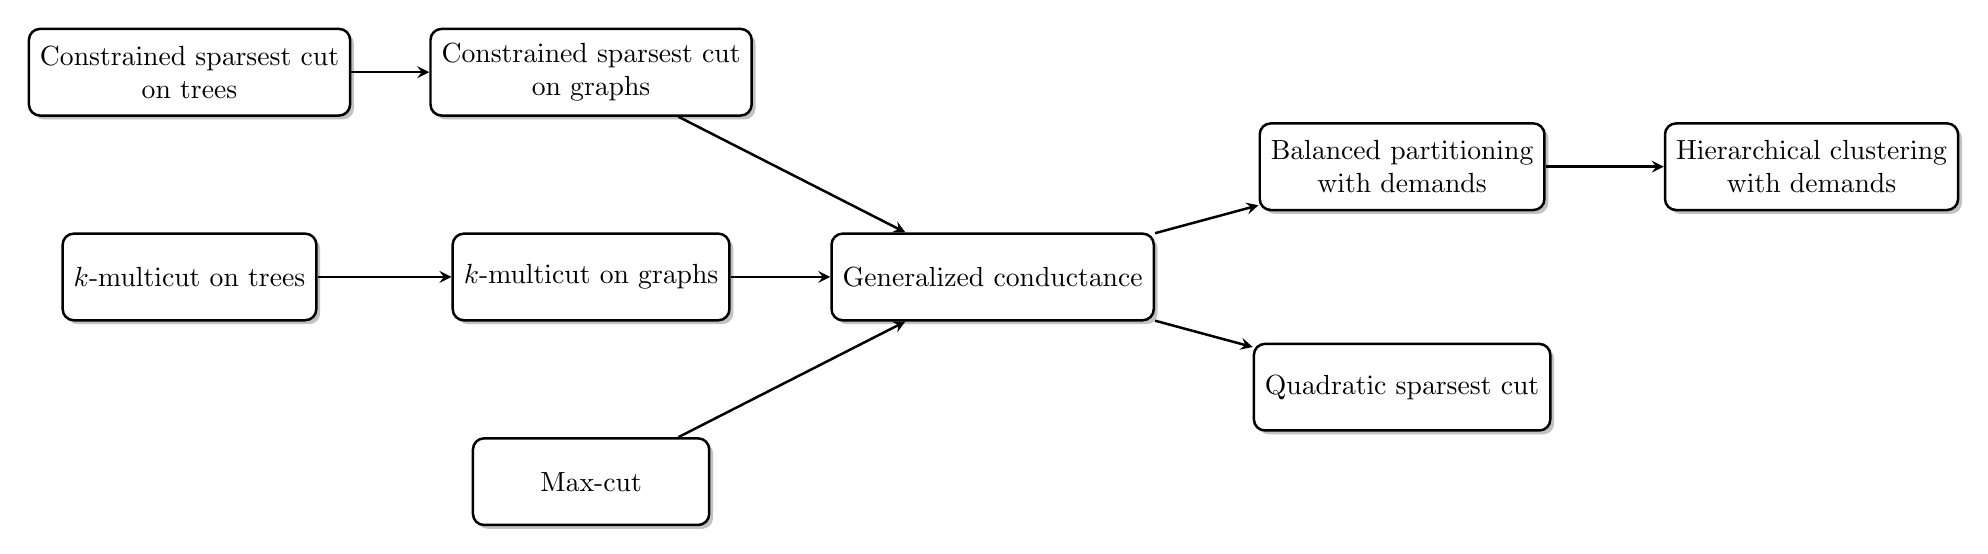
\begin{tikzpicture}[>=stealth, line width=0.9pt]
  \tikzstyle{box}=[draw, rounded corners, align=center, inner sep=4pt,
    minimum width=3cm, minimum height=1.10cm,
    fill=white,
    preaction={fill=black,opacity=0.24,transform canvas={xshift=1.4pt,yshift=-1.4pt}}]

  % Left: tree problems
  \node[box] (cst) at (0, 2.6) {Constrained sparsest cut\\on trees};
  \node[box] (kmt) at (0, 0.0) {$k$-multicut on trees};

  % Middle-left: graph problems + max-cut
  \node[box] (csg) at (5.1, 2.6) {Constrained sparsest cut\\on graphs};
  \node[box] (kmg) at (5.1, 0.0) {$k$-multicut on graphs};
  \node[box] (mc)  at (5.1, -2.6) {Max-cut};

  % Center: target problem
  \node[box, minimum width=3cm] (gc) at (10.2, 0.0) {Generalized conductance};

  % Right: applications
  \node[box] (bpd) at (15.4, 1.4) {Balanced partitioning\\with demands};
  \node[box] (qsc) at (15.4, -1.4) {Quadratic sparsest cut};
  \node[box] (hcd) at (20.6, 1.4) {Hierarchical clustering\\with demands};

  \draw[->] (cst) -- (csg);
  \draw[->] (kmt) -- (kmg);

  \draw[->] (csg) -- (gc);
  \draw[->] (kmg) -- (gc);
  \draw[->] (mc)  -- (gc);

  \draw[->] (gc) -- (bpd);
  \draw[->] (gc) -- (qsc);
  \draw[->] (bpd) -- (hcd);
\end{tikzpicture}
